% Options for packages loaded elsewhere
\PassOptionsToPackage{unicode}{hyperref}
\PassOptionsToPackage{hyphens}{url}
%
\documentclass[
]{article}
\usepackage{amsmath,amssymb}
\usepackage{iftex}
\ifPDFTeX
  \usepackage[T1]{fontenc}
  \usepackage[utf8]{inputenc}
  \usepackage{textcomp} % provide euro and other symbols
\else % if luatex or xetex
  \usepackage{unicode-math} % this also loads fontspec
  \defaultfontfeatures{Scale=MatchLowercase}
  \defaultfontfeatures[\rmfamily]{Ligatures=TeX,Scale=1}
\fi
\usepackage{lmodern}
\ifPDFTeX\else
  % xetex/luatex font selection
\fi
% Use upquote if available, for straight quotes in verbatim environments
\IfFileExists{upquote.sty}{\usepackage{upquote}}{}
\IfFileExists{microtype.sty}{% use microtype if available
  \usepackage[]{microtype}
  \UseMicrotypeSet[protrusion]{basicmath} % disable protrusion for tt fonts
}{}
\makeatletter
\@ifundefined{KOMAClassName}{% if non-KOMA class
  \IfFileExists{parskip.sty}{%
    \usepackage{parskip}
  }{% else
    \setlength{\parindent}{0pt}
    \setlength{\parskip}{6pt plus 2pt minus 1pt}}
}{% if KOMA class
  \KOMAoptions{parskip=half}}
\makeatother
\usepackage{xcolor}
\usepackage[margin=1in]{geometry}
\usepackage{color}
\usepackage{fancyvrb}
\newcommand{\VerbBar}{|}
\newcommand{\VERB}{\Verb[commandchars=\\\{\}]}
\DefineVerbatimEnvironment{Highlighting}{Verbatim}{commandchars=\\\{\}}
% Add ',fontsize=\small' for more characters per line
\usepackage{framed}
\definecolor{shadecolor}{RGB}{248,248,248}
\newenvironment{Shaded}{\begin{snugshade}}{\end{snugshade}}
\newcommand{\AlertTok}[1]{\textcolor[rgb]{0.94,0.16,0.16}{#1}}
\newcommand{\AnnotationTok}[1]{\textcolor[rgb]{0.56,0.35,0.01}{\textbf{\textit{#1}}}}
\newcommand{\AttributeTok}[1]{\textcolor[rgb]{0.13,0.29,0.53}{#1}}
\newcommand{\BaseNTok}[1]{\textcolor[rgb]{0.00,0.00,0.81}{#1}}
\newcommand{\BuiltInTok}[1]{#1}
\newcommand{\CharTok}[1]{\textcolor[rgb]{0.31,0.60,0.02}{#1}}
\newcommand{\CommentTok}[1]{\textcolor[rgb]{0.56,0.35,0.01}{\textit{#1}}}
\newcommand{\CommentVarTok}[1]{\textcolor[rgb]{0.56,0.35,0.01}{\textbf{\textit{#1}}}}
\newcommand{\ConstantTok}[1]{\textcolor[rgb]{0.56,0.35,0.01}{#1}}
\newcommand{\ControlFlowTok}[1]{\textcolor[rgb]{0.13,0.29,0.53}{\textbf{#1}}}
\newcommand{\DataTypeTok}[1]{\textcolor[rgb]{0.13,0.29,0.53}{#1}}
\newcommand{\DecValTok}[1]{\textcolor[rgb]{0.00,0.00,0.81}{#1}}
\newcommand{\DocumentationTok}[1]{\textcolor[rgb]{0.56,0.35,0.01}{\textbf{\textit{#1}}}}
\newcommand{\ErrorTok}[1]{\textcolor[rgb]{0.64,0.00,0.00}{\textbf{#1}}}
\newcommand{\ExtensionTok}[1]{#1}
\newcommand{\FloatTok}[1]{\textcolor[rgb]{0.00,0.00,0.81}{#1}}
\newcommand{\FunctionTok}[1]{\textcolor[rgb]{0.13,0.29,0.53}{\textbf{#1}}}
\newcommand{\ImportTok}[1]{#1}
\newcommand{\InformationTok}[1]{\textcolor[rgb]{0.56,0.35,0.01}{\textbf{\textit{#1}}}}
\newcommand{\KeywordTok}[1]{\textcolor[rgb]{0.13,0.29,0.53}{\textbf{#1}}}
\newcommand{\NormalTok}[1]{#1}
\newcommand{\OperatorTok}[1]{\textcolor[rgb]{0.81,0.36,0.00}{\textbf{#1}}}
\newcommand{\OtherTok}[1]{\textcolor[rgb]{0.56,0.35,0.01}{#1}}
\newcommand{\PreprocessorTok}[1]{\textcolor[rgb]{0.56,0.35,0.01}{\textit{#1}}}
\newcommand{\RegionMarkerTok}[1]{#1}
\newcommand{\SpecialCharTok}[1]{\textcolor[rgb]{0.81,0.36,0.00}{\textbf{#1}}}
\newcommand{\SpecialStringTok}[1]{\textcolor[rgb]{0.31,0.60,0.02}{#1}}
\newcommand{\StringTok}[1]{\textcolor[rgb]{0.31,0.60,0.02}{#1}}
\newcommand{\VariableTok}[1]{\textcolor[rgb]{0.00,0.00,0.00}{#1}}
\newcommand{\VerbatimStringTok}[1]{\textcolor[rgb]{0.31,0.60,0.02}{#1}}
\newcommand{\WarningTok}[1]{\textcolor[rgb]{0.56,0.35,0.01}{\textbf{\textit{#1}}}}
\usepackage{longtable,booktabs,array}
\usepackage{calc} % for calculating minipage widths
% Correct order of tables after \paragraph or \subparagraph
\usepackage{etoolbox}
\makeatletter
\patchcmd\longtable{\par}{\if@noskipsec\mbox{}\fi\par}{}{}
\makeatother
% Allow footnotes in longtable head/foot
\IfFileExists{footnotehyper.sty}{\usepackage{footnotehyper}}{\usepackage{footnote}}
\makesavenoteenv{longtable}
\usepackage{graphicx}
\makeatletter
\def\maxwidth{\ifdim\Gin@nat@width>\linewidth\linewidth\else\Gin@nat@width\fi}
\def\maxheight{\ifdim\Gin@nat@height>\textheight\textheight\else\Gin@nat@height\fi}
\makeatother
% Scale images if necessary, so that they will not overflow the page
% margins by default, and it is still possible to overwrite the defaults
% using explicit options in \includegraphics[width, height, ...]{}
\setkeys{Gin}{width=\maxwidth,height=\maxheight,keepaspectratio}
% Set default figure placement to htbp
\makeatletter
\def\fps@figure{htbp}
\makeatother
\setlength{\emergencystretch}{3em} % prevent overfull lines
\providecommand{\tightlist}{%
  \setlength{\itemsep}{0pt}\setlength{\parskip}{0pt}}
\setcounter{secnumdepth}{-\maxdimen} % remove section numbering
\ifLuaTeX
  \usepackage{selnolig}  % disable illegal ligatures
\fi
\IfFileExists{bookmark.sty}{\usepackage{bookmark}}{\usepackage{hyperref}}
\IfFileExists{xurl.sty}{\usepackage{xurl}}{} % add URL line breaks if available
\urlstyle{same}
\hypersetup{
  pdftitle={Class10: Halloween Candy Mini Project},
  pdfauthor={Brittney Hayes},
  hidelinks,
  pdfcreator={LaTeX via pandoc}}

\title{Class10: Halloween Candy Mini Project}
\author{Brittney Hayes}
\date{2024-02-12}

\begin{document}
\maketitle

\hypertarget{importing-candy-data}{%
\section{1. Importing Candy Data}\label{importing-candy-data}}

\begin{Shaded}
\begin{Highlighting}[]
\NormalTok{candy\_data }\OtherTok{\textless{}{-}} \FunctionTok{read.csv}\NormalTok{(}\StringTok{"https://raw.githubusercontent.com/fivethirtyeight/data/master/candy{-}power{-}ranking/candy{-}data.csv"}\NormalTok{) }
\NormalTok{candy\_file }\OtherTok{\textless{}{-}}\NormalTok{ candy\_data}
\end{Highlighting}
\end{Shaded}

Q1. How many different candy types are in this dataset?

\begin{Shaded}
\begin{Highlighting}[]
\FunctionTok{dim}\NormalTok{(candy\_file)}
\end{Highlighting}
\end{Shaded}

\begin{verbatim}
## [1] 85 13
\end{verbatim}

\begin{Shaded}
\begin{Highlighting}[]
\FunctionTok{ncol}\NormalTok{(candy\_file[}\DecValTok{2}\SpecialCharTok{:}\DecValTok{10}\NormalTok{])}
\end{Highlighting}
\end{Shaded}

\begin{verbatim}
## [1] 9
\end{verbatim}

There are 85 brands of candy and 9 types, I omitted a few columns that
were not specifying types of candy.

Q2. How many fruity candy types are in the dataset?

\begin{Shaded}
\begin{Highlighting}[]
\FunctionTok{sum}\NormalTok{(candy\_file[}\StringTok{"fruity"}\NormalTok{])}
\end{Highlighting}
\end{Shaded}

\begin{verbatim}
## [1] 38
\end{verbatim}

There are 38 fruity candy types.

\hypertarget{what-is-your-favorite-candy}{%
\section{2. What is your favorite
candy?}\label{what-is-your-favorite-candy}}

Q3. What is your favorite candy in the dataset and what is it's
winpercent value?

\begin{Shaded}
\begin{Highlighting}[]
\NormalTok{candy\_file[}\DecValTok{65}\NormalTok{,]}\SpecialCharTok{$}\NormalTok{winpercent}
\end{Highlighting}
\end{Shaded}

\begin{verbatim}
## [1] 76.67378
\end{verbatim}

My favorite candy is Snickers and the winpercent value is 76.67378.

Q4. What is the winpercent value for ``Kit Kat''?

\begin{Shaded}
\begin{Highlighting}[]
\NormalTok{candy\_file[}\DecValTok{29}\NormalTok{,]}\SpecialCharTok{$}\NormalTok{winpercent}
\end{Highlighting}
\end{Shaded}

\begin{verbatim}
## [1] 76.7686
\end{verbatim}

Q5. What is the winpercent value for ``Tootsie Roll Snack Bars''?

\begin{Shaded}
\begin{Highlighting}[]
\NormalTok{candy\_file[}\DecValTok{78}\NormalTok{,]}\SpecialCharTok{$}\NormalTok{winpercent}
\end{Highlighting}
\end{Shaded}

\begin{verbatim}
## [1] 49.6535
\end{verbatim}

\begin{Shaded}
\begin{Highlighting}[]
\CommentTok{\#install.packages("skimr")}
\FunctionTok{library}\NormalTok{(}\StringTok{"skimr"}\NormalTok{)}
\FunctionTok{skim}\NormalTok{(candy\_file)}
\end{Highlighting}
\end{Shaded}

\begin{longtable}[]{@{}ll@{}}
\caption{Data summary}\tabularnewline
\toprule\noalign{}
\endfirsthead
\endhead
\bottomrule\noalign{}
\endlastfoot
Name & candy\_file \\
Number of rows & 85 \\
Number of columns & 13 \\
\_\_\_\_\_\_\_\_\_\_\_\_\_\_\_\_\_\_\_\_\_\_\_ & \\
Column type frequency: & \\
character & 1 \\
numeric & 12 \\
\_\_\_\_\_\_\_\_\_\_\_\_\_\_\_\_\_\_\_\_\_\_\_\_ & \\
Group variables & None \\
\end{longtable}

\textbf{Variable type: character}

\begin{longtable}[]{@{}
  >{\raggedright\arraybackslash}p{(\columnwidth - 14\tabcolsep) * \real{0.2055}}
  >{\raggedleft\arraybackslash}p{(\columnwidth - 14\tabcolsep) * \real{0.1370}}
  >{\raggedleft\arraybackslash}p{(\columnwidth - 14\tabcolsep) * \real{0.1918}}
  >{\raggedleft\arraybackslash}p{(\columnwidth - 14\tabcolsep) * \real{0.0548}}
  >{\raggedleft\arraybackslash}p{(\columnwidth - 14\tabcolsep) * \real{0.0548}}
  >{\raggedleft\arraybackslash}p{(\columnwidth - 14\tabcolsep) * \real{0.0822}}
  >{\raggedleft\arraybackslash}p{(\columnwidth - 14\tabcolsep) * \real{0.1233}}
  >{\raggedleft\arraybackslash}p{(\columnwidth - 14\tabcolsep) * \real{0.1507}}@{}}
\toprule\noalign{}
\begin{minipage}[b]{\linewidth}\raggedright
skim\_variable
\end{minipage} & \begin{minipage}[b]{\linewidth}\raggedleft
n\_missing
\end{minipage} & \begin{minipage}[b]{\linewidth}\raggedleft
complete\_rate
\end{minipage} & \begin{minipage}[b]{\linewidth}\raggedleft
min
\end{minipage} & \begin{minipage}[b]{\linewidth}\raggedleft
max
\end{minipage} & \begin{minipage}[b]{\linewidth}\raggedleft
empty
\end{minipage} & \begin{minipage}[b]{\linewidth}\raggedleft
n\_unique
\end{minipage} & \begin{minipage}[b]{\linewidth}\raggedleft
whitespace
\end{minipage} \\
\midrule\noalign{}
\endhead
\bottomrule\noalign{}
\endlastfoot
competitorname & 0 & 1 & 4 & 27 & 0 & 85 & 0 \\
\end{longtable}

\textbf{Variable type: numeric}

\begin{longtable}[]{@{}
  >{\raggedright\arraybackslash}p{(\columnwidth - 20\tabcolsep) * \real{0.1910}}
  >{\raggedleft\arraybackslash}p{(\columnwidth - 20\tabcolsep) * \real{0.1124}}
  >{\raggedleft\arraybackslash}p{(\columnwidth - 20\tabcolsep) * \real{0.1573}}
  >{\raggedleft\arraybackslash}p{(\columnwidth - 20\tabcolsep) * \real{0.0674}}
  >{\raggedleft\arraybackslash}p{(\columnwidth - 20\tabcolsep) * \real{0.0674}}
  >{\raggedleft\arraybackslash}p{(\columnwidth - 20\tabcolsep) * \real{0.0674}}
  >{\raggedleft\arraybackslash}p{(\columnwidth - 20\tabcolsep) * \real{0.0674}}
  >{\raggedleft\arraybackslash}p{(\columnwidth - 20\tabcolsep) * \real{0.0674}}
  >{\raggedleft\arraybackslash}p{(\columnwidth - 20\tabcolsep) * \real{0.0674}}
  >{\raggedleft\arraybackslash}p{(\columnwidth - 20\tabcolsep) * \real{0.0674}}
  >{\raggedright\arraybackslash}p{(\columnwidth - 20\tabcolsep) * \real{0.0674}}@{}}
\toprule\noalign{}
\begin{minipage}[b]{\linewidth}\raggedright
skim\_variable
\end{minipage} & \begin{minipage}[b]{\linewidth}\raggedleft
n\_missing
\end{minipage} & \begin{minipage}[b]{\linewidth}\raggedleft
complete\_rate
\end{minipage} & \begin{minipage}[b]{\linewidth}\raggedleft
mean
\end{minipage} & \begin{minipage}[b]{\linewidth}\raggedleft
sd
\end{minipage} & \begin{minipage}[b]{\linewidth}\raggedleft
p0
\end{minipage} & \begin{minipage}[b]{\linewidth}\raggedleft
p25
\end{minipage} & \begin{minipage}[b]{\linewidth}\raggedleft
p50
\end{minipage} & \begin{minipage}[b]{\linewidth}\raggedleft
p75
\end{minipage} & \begin{minipage}[b]{\linewidth}\raggedleft
p100
\end{minipage} & \begin{minipage}[b]{\linewidth}\raggedright
hist
\end{minipage} \\
\midrule\noalign{}
\endhead
\bottomrule\noalign{}
\endlastfoot
chocolate & 0 & 1 & 0.44 & 0.50 & 0.00 & 0.00 & 0.00 & 1.00 & 1.00 &
▇▁▁▁▆ \\
fruity & 0 & 1 & 0.45 & 0.50 & 0.00 & 0.00 & 0.00 & 1.00 & 1.00 &
▇▁▁▁▆ \\
caramel & 0 & 1 & 0.16 & 0.37 & 0.00 & 0.00 & 0.00 & 0.00 & 1.00 &
▇▁▁▁▂ \\
peanutyalmondy & 0 & 1 & 0.16 & 0.37 & 0.00 & 0.00 & 0.00 & 0.00 & 1.00
& ▇▁▁▁▂ \\
nougat & 0 & 1 & 0.08 & 0.28 & 0.00 & 0.00 & 0.00 & 0.00 & 1.00 &
▇▁▁▁▁ \\
crispedricewafer & 0 & 1 & 0.08 & 0.28 & 0.00 & 0.00 & 0.00 & 0.00 &
1.00 & ▇▁▁▁▁ \\
hard & 0 & 1 & 0.18 & 0.38 & 0.00 & 0.00 & 0.00 & 0.00 & 1.00 & ▇▁▁▁▂ \\
bar & 0 & 1 & 0.25 & 0.43 & 0.00 & 0.00 & 0.00 & 0.00 & 1.00 & ▇▁▁▁▂ \\
pluribus & 0 & 1 & 0.52 & 0.50 & 0.00 & 0.00 & 1.00 & 1.00 & 1.00 &
▇▁▁▁▇ \\
sugarpercent & 0 & 1 & 0.48 & 0.28 & 0.01 & 0.22 & 0.47 & 0.73 & 0.99 &
▇▇▇▇▆ \\
pricepercent & 0 & 1 & 0.47 & 0.29 & 0.01 & 0.26 & 0.47 & 0.65 & 0.98 &
▇▇▇▇▆ \\
winpercent & 0 & 1 & 50.32 & 14.71 & 22.45 & 39.14 & 47.83 & 59.86 &
84.18 & ▃▇▆▅▂ \\
\end{longtable}

Q6. Is there any variable/column that looks to be on a different scale
to the majority of the other columns in the dataset?

\begin{Shaded}
\begin{Highlighting}[]
\FunctionTok{library}\NormalTok{(skimr)}
\FunctionTok{skim}\NormalTok{(candy\_file)}
\end{Highlighting}
\end{Shaded}

\begin{longtable}[]{@{}ll@{}}
\caption{Data summary}\tabularnewline
\toprule\noalign{}
\endfirsthead
\endhead
\bottomrule\noalign{}
\endlastfoot
Name & candy\_file \\
Number of rows & 85 \\
Number of columns & 13 \\
\_\_\_\_\_\_\_\_\_\_\_\_\_\_\_\_\_\_\_\_\_\_\_ & \\
Column type frequency: & \\
character & 1 \\
numeric & 12 \\
\_\_\_\_\_\_\_\_\_\_\_\_\_\_\_\_\_\_\_\_\_\_\_\_ & \\
Group variables & None \\
\end{longtable}

\textbf{Variable type: character}

\begin{longtable}[]{@{}
  >{\raggedright\arraybackslash}p{(\columnwidth - 14\tabcolsep) * \real{0.2055}}
  >{\raggedleft\arraybackslash}p{(\columnwidth - 14\tabcolsep) * \real{0.1370}}
  >{\raggedleft\arraybackslash}p{(\columnwidth - 14\tabcolsep) * \real{0.1918}}
  >{\raggedleft\arraybackslash}p{(\columnwidth - 14\tabcolsep) * \real{0.0548}}
  >{\raggedleft\arraybackslash}p{(\columnwidth - 14\tabcolsep) * \real{0.0548}}
  >{\raggedleft\arraybackslash}p{(\columnwidth - 14\tabcolsep) * \real{0.0822}}
  >{\raggedleft\arraybackslash}p{(\columnwidth - 14\tabcolsep) * \real{0.1233}}
  >{\raggedleft\arraybackslash}p{(\columnwidth - 14\tabcolsep) * \real{0.1507}}@{}}
\toprule\noalign{}
\begin{minipage}[b]{\linewidth}\raggedright
skim\_variable
\end{minipage} & \begin{minipage}[b]{\linewidth}\raggedleft
n\_missing
\end{minipage} & \begin{minipage}[b]{\linewidth}\raggedleft
complete\_rate
\end{minipage} & \begin{minipage}[b]{\linewidth}\raggedleft
min
\end{minipage} & \begin{minipage}[b]{\linewidth}\raggedleft
max
\end{minipage} & \begin{minipage}[b]{\linewidth}\raggedleft
empty
\end{minipage} & \begin{minipage}[b]{\linewidth}\raggedleft
n\_unique
\end{minipage} & \begin{minipage}[b]{\linewidth}\raggedleft
whitespace
\end{minipage} \\
\midrule\noalign{}
\endhead
\bottomrule\noalign{}
\endlastfoot
competitorname & 0 & 1 & 4 & 27 & 0 & 85 & 0 \\
\end{longtable}

\textbf{Variable type: numeric}

\begin{longtable}[]{@{}
  >{\raggedright\arraybackslash}p{(\columnwidth - 20\tabcolsep) * \real{0.1910}}
  >{\raggedleft\arraybackslash}p{(\columnwidth - 20\tabcolsep) * \real{0.1124}}
  >{\raggedleft\arraybackslash}p{(\columnwidth - 20\tabcolsep) * \real{0.1573}}
  >{\raggedleft\arraybackslash}p{(\columnwidth - 20\tabcolsep) * \real{0.0674}}
  >{\raggedleft\arraybackslash}p{(\columnwidth - 20\tabcolsep) * \real{0.0674}}
  >{\raggedleft\arraybackslash}p{(\columnwidth - 20\tabcolsep) * \real{0.0674}}
  >{\raggedleft\arraybackslash}p{(\columnwidth - 20\tabcolsep) * \real{0.0674}}
  >{\raggedleft\arraybackslash}p{(\columnwidth - 20\tabcolsep) * \real{0.0674}}
  >{\raggedleft\arraybackslash}p{(\columnwidth - 20\tabcolsep) * \real{0.0674}}
  >{\raggedleft\arraybackslash}p{(\columnwidth - 20\tabcolsep) * \real{0.0674}}
  >{\raggedright\arraybackslash}p{(\columnwidth - 20\tabcolsep) * \real{0.0674}}@{}}
\toprule\noalign{}
\begin{minipage}[b]{\linewidth}\raggedright
skim\_variable
\end{minipage} & \begin{minipage}[b]{\linewidth}\raggedleft
n\_missing
\end{minipage} & \begin{minipage}[b]{\linewidth}\raggedleft
complete\_rate
\end{minipage} & \begin{minipage}[b]{\linewidth}\raggedleft
mean
\end{minipage} & \begin{minipage}[b]{\linewidth}\raggedleft
sd
\end{minipage} & \begin{minipage}[b]{\linewidth}\raggedleft
p0
\end{minipage} & \begin{minipage}[b]{\linewidth}\raggedleft
p25
\end{minipage} & \begin{minipage}[b]{\linewidth}\raggedleft
p50
\end{minipage} & \begin{minipage}[b]{\linewidth}\raggedleft
p75
\end{minipage} & \begin{minipage}[b]{\linewidth}\raggedleft
p100
\end{minipage} & \begin{minipage}[b]{\linewidth}\raggedright
hist
\end{minipage} \\
\midrule\noalign{}
\endhead
\bottomrule\noalign{}
\endlastfoot
chocolate & 0 & 1 & 0.44 & 0.50 & 0.00 & 0.00 & 0.00 & 1.00 & 1.00 &
▇▁▁▁▆ \\
fruity & 0 & 1 & 0.45 & 0.50 & 0.00 & 0.00 & 0.00 & 1.00 & 1.00 &
▇▁▁▁▆ \\
caramel & 0 & 1 & 0.16 & 0.37 & 0.00 & 0.00 & 0.00 & 0.00 & 1.00 &
▇▁▁▁▂ \\
peanutyalmondy & 0 & 1 & 0.16 & 0.37 & 0.00 & 0.00 & 0.00 & 0.00 & 1.00
& ▇▁▁▁▂ \\
nougat & 0 & 1 & 0.08 & 0.28 & 0.00 & 0.00 & 0.00 & 0.00 & 1.00 &
▇▁▁▁▁ \\
crispedricewafer & 0 & 1 & 0.08 & 0.28 & 0.00 & 0.00 & 0.00 & 0.00 &
1.00 & ▇▁▁▁▁ \\
hard & 0 & 1 & 0.18 & 0.38 & 0.00 & 0.00 & 0.00 & 0.00 & 1.00 & ▇▁▁▁▂ \\
bar & 0 & 1 & 0.25 & 0.43 & 0.00 & 0.00 & 0.00 & 0.00 & 1.00 & ▇▁▁▁▂ \\
pluribus & 0 & 1 & 0.52 & 0.50 & 0.00 & 0.00 & 1.00 & 1.00 & 1.00 &
▇▁▁▁▇ \\
sugarpercent & 0 & 1 & 0.48 & 0.28 & 0.01 & 0.22 & 0.47 & 0.73 & 0.99 &
▇▇▇▇▆ \\
pricepercent & 0 & 1 & 0.47 & 0.29 & 0.01 & 0.26 & 0.47 & 0.65 & 0.98 &
▇▇▇▇▆ \\
winpercent & 0 & 1 & 50.32 & 14.71 & 22.45 & 39.14 & 47.83 & 59.86 &
84.18 & ▃▇▆▅▂ \\
\end{longtable}

Sugarpercent, pricepercent, and winpercent appear different.

Q7. What do you think a zero and one represent for the candy\$chocolate
column?

\begin{Shaded}
\begin{Highlighting}[]
\FunctionTok{table}\NormalTok{(candy\_file}\SpecialCharTok{$}\NormalTok{chocolate)}
\end{Highlighting}
\end{Shaded}

\begin{verbatim}
## 
##  0  1 
## 48 37
\end{verbatim}

The 0 and 1 confirm if the candy type falls into this candy, 0 means it
does not/false and 1 means it does/true.

\hypertarget{overall-candy-rankings}{%
\section{3. Overall Candy Rankings}\label{overall-candy-rankings}}

Q8. Plot a histogram of winpercent values

\begin{Shaded}
\begin{Highlighting}[]
\FunctionTok{hist}\NormalTok{(candy\_data}\SpecialCharTok{$}\NormalTok{winpercent, }
     \AttributeTok{main =} \StringTok{"Histogram of Winpercent Values"}\NormalTok{,}
     \AttributeTok{xlab =} \StringTok{"Winpercent"}\NormalTok{,}
     \AttributeTok{ylab =} \StringTok{"Frequency"}\NormalTok{)}
\end{Highlighting}
\end{Shaded}

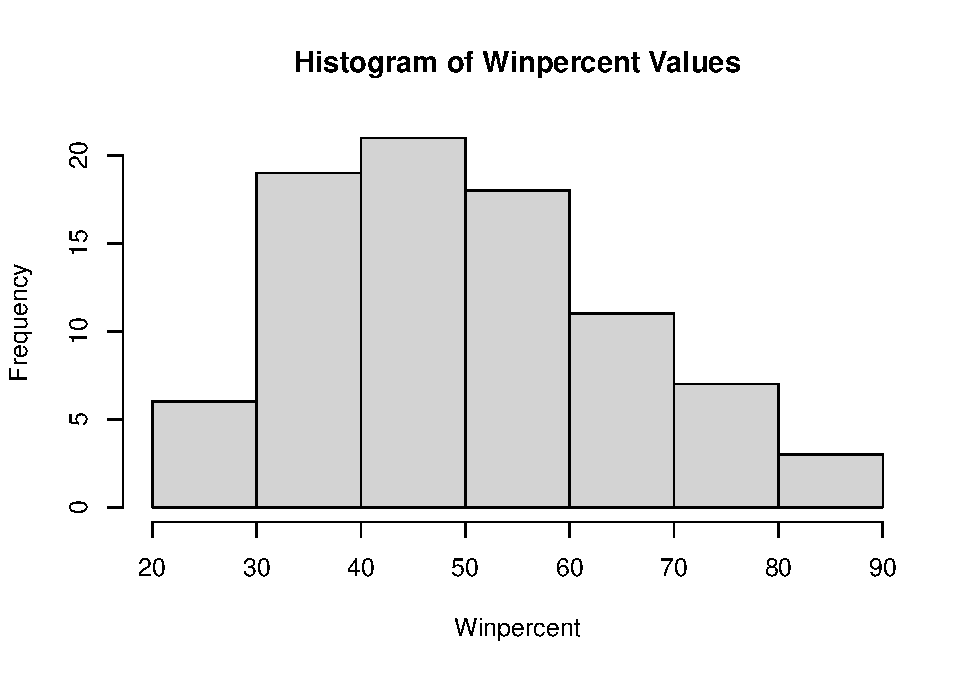
\includegraphics{Untitled_files/figure-latex/unnamed-chunk-11-1.pdf}

Q9. Is the distribution of winpercent values symmetrical? Based on the
appearance of the histogram, no.

Q10. Is the center of the distribution above or below 50\%?

\begin{Shaded}
\begin{Highlighting}[]
\FunctionTok{mean}\NormalTok{(candy\_file}\SpecialCharTok{$}\NormalTok{winpercent)}
\end{Highlighting}
\end{Shaded}

\begin{verbatim}
## [1] 50.31676
\end{verbatim}

\begin{Shaded}
\begin{Highlighting}[]
\FunctionTok{median}\NormalTok{(candy\_file}\SpecialCharTok{$}\NormalTok{winpercent)}
\end{Highlighting}
\end{Shaded}

\begin{verbatim}
## [1] 47.82975
\end{verbatim}

Based on the mean, it's above 50\% but by very little. Based on the
median, it's below 50\% again by little. Based on the histogram it
appears below 50\%. So I would say below 50\%.

Q11. On average is chocolate candy higher or lower ranked than fruit
candy?

\begin{Shaded}
\begin{Highlighting}[]
\NormalTok{candy\_file}\SpecialCharTok{$}\NormalTok{winpercent[}\FunctionTok{as.logical}\NormalTok{(candy\_file}\SpecialCharTok{$}\NormalTok{chocolate)]}
\end{Highlighting}
\end{Shaded}

\begin{verbatim}
##  [1] 66.97173 67.60294 50.34755 56.91455 38.97504 55.37545 62.28448 56.49050
##  [9] 59.23612 57.21925 76.76860 71.46505 66.57458 55.06407 73.09956 60.80070
## [17] 64.35334 47.82975 54.52645 70.73564 66.47068 69.48379 81.86626 84.18029
## [25] 73.43499 72.88790 65.71629 34.72200 37.88719 76.67378 59.52925 48.98265
## [33] 43.06890 45.73675 49.65350 81.64291 49.52411
\end{verbatim}

\begin{Shaded}
\begin{Highlighting}[]
\FunctionTok{mean}\NormalTok{(candy\_file}\SpecialCharTok{$}\NormalTok{winpercent[}\FunctionTok{as.logical}\NormalTok{(candy\_file}\SpecialCharTok{$}\NormalTok{chocolate)])}
\end{Highlighting}
\end{Shaded}

\begin{verbatim}
## [1] 60.92153
\end{verbatim}

\begin{Shaded}
\begin{Highlighting}[]
\NormalTok{candy\_file}\SpecialCharTok{$}\NormalTok{winpercent[}\FunctionTok{as.logical}\NormalTok{(candy\_file}\SpecialCharTok{$}\NormalTok{fruity)]}
\end{Highlighting}
\end{Shaded}

\begin{verbatim}
##  [1] 52.34146 34.51768 36.01763 24.52499 42.27208 39.46056 43.08892 39.18550
##  [9] 46.78335 57.11974 51.41243 42.17877 28.12744 41.38956 39.14106 52.91139
## [17] 46.41172 55.35405 22.44534 39.44680 41.26551 37.34852 35.29076 42.84914
## [25] 63.08514 55.10370 45.99583 59.86400 52.82595 67.03763 34.57899 27.30386
## [33] 54.86111 48.98265 47.17323 45.46628 39.01190 44.37552
\end{verbatim}

\begin{Shaded}
\begin{Highlighting}[]
\FunctionTok{mean}\NormalTok{(candy\_file}\SpecialCharTok{$}\NormalTok{winpercent[}\FunctionTok{as.logical}\NormalTok{(candy\_file}\SpecialCharTok{$}\NormalTok{fruity)])}
\end{Highlighting}
\end{Shaded}

\begin{verbatim}
## [1] 44.11974
\end{verbatim}

Chocolate candy is ranked higher than fruity candy on average.

Q12. Is this difference statistically significant?

\begin{Shaded}
\begin{Highlighting}[]
\NormalTok{chocolate }\OtherTok{\textless{}{-}}\NormalTok{ candy\_file}\SpecialCharTok{$}\NormalTok{winpercent[}\FunctionTok{as.logical}\NormalTok{(candy\_file}\SpecialCharTok{$}\NormalTok{chocolate)]}
\NormalTok{fruit }\OtherTok{\textless{}{-}}\NormalTok{ candy\_file}\SpecialCharTok{$}\NormalTok{winpercent[}\FunctionTok{as.logical}\NormalTok{(candy\_file}\SpecialCharTok{$}\NormalTok{fruity)]}

\FunctionTok{t.test}\NormalTok{(chocolate,fruit)}
\end{Highlighting}
\end{Shaded}

\begin{verbatim}
## 
##  Welch Two Sample t-test
## 
## data:  chocolate and fruit
## t = 6.2582, df = 68.882, p-value = 2.871e-08
## alternative hypothesis: true difference in means is not equal to 0
## 95 percent confidence interval:
##  11.44563 22.15795
## sample estimates:
## mean of x mean of y 
##  60.92153  44.11974
\end{verbatim}

Since the p-value is less than 0.05, yes the difference is statistically
significant.

Q13. What are the five least liked candy types in this set?

\begin{Shaded}
\begin{Highlighting}[]
\FunctionTok{head}\NormalTok{(candy\_file[}\FunctionTok{order}\NormalTok{(candy\_file}\SpecialCharTok{$}\NormalTok{winpercent),], }\AttributeTok{n=}\DecValTok{5}\NormalTok{)}
\end{Highlighting}
\end{Shaded}

\begin{verbatim}
##        competitorname chocolate fruity caramel peanutyalmondy nougat
## 45          Nik L Nip         0      1       0              0      0
## 8  Boston Baked Beans         0      0       0              1      0
## 13           Chiclets         0      1       0              0      0
## 73       Super Bubble         0      1       0              0      0
## 27         Jawbusters         0      1       0              0      0
##    crispedricewafer hard bar pluribus sugarpercent pricepercent winpercent
## 45                0    0   0        1        0.197        0.976   22.44534
## 8                 0    0   0        1        0.313        0.511   23.41782
## 13                0    0   0        1        0.046        0.325   24.52499
## 73                0    0   0        0        0.162        0.116   27.30386
## 27                0    1   0        1        0.093        0.511   28.12744
\end{verbatim}

The 5 least liked candy types are Nik L Nip, Boston Baked Beans,
Chiclets, Super Bubble, and Jawbusters.

Q14. What are the top 5 all time favorite candy types out of this set?

\begin{Shaded}
\begin{Highlighting}[]
\FunctionTok{tail}\NormalTok{(candy\_file[}\FunctionTok{order}\NormalTok{(candy\_file}\SpecialCharTok{$}\NormalTok{winpercent),], }\AttributeTok{n=}\DecValTok{5}\NormalTok{)}
\end{Highlighting}
\end{Shaded}

\begin{verbatim}
##               competitorname chocolate fruity caramel peanutyalmondy nougat
## 65                  Snickers         1      0       1              1      1
## 29                   Kit Kat         1      0       0              0      0
## 80                      Twix         1      0       1              0      0
## 52        Reese's Miniatures         1      0       0              1      0
## 53 Reese's Peanut Butter cup         1      0       0              1      0
##    crispedricewafer hard bar pluribus sugarpercent pricepercent winpercent
## 65                0    0   1        0        0.546        0.651   76.67378
## 29                1    0   1        0        0.313        0.511   76.76860
## 80                1    0   1        0        0.546        0.906   81.64291
## 52                0    0   0        0        0.034        0.279   81.86626
## 53                0    0   0        0        0.720        0.651   84.18029
\end{verbatim}

The top 5 all time favorite candy types are Reese's Peanut Butter cup,
Reese's Miniatures, Twix, Kit Kat, and Snickers.

Q15. Make a first barplot of candy ranking based on winpercent values.

\begin{Shaded}
\begin{Highlighting}[]
\CommentTok{\#install.packages("ggplot2")}
\FunctionTok{library}\NormalTok{(ggplot2)}

\FunctionTok{ggplot}\NormalTok{(candy\_file) }\SpecialCharTok{+} 
  \FunctionTok{aes}\NormalTok{(}\AttributeTok{x =}\NormalTok{ winpercent, }\AttributeTok{y =} \FunctionTok{rownames}\NormalTok{(candy\_file)) }\SpecialCharTok{+}
  \FunctionTok{geom\_bar}\NormalTok{(}\AttributeTok{stat =} \StringTok{"identity"}\NormalTok{, }\AttributeTok{fill =} \StringTok{"grey"}\NormalTok{) }\SpecialCharTok{+}
  \FunctionTok{labs}\NormalTok{(}\AttributeTok{x =} \StringTok{"winpercent"}\NormalTok{, }\AttributeTok{y =} \StringTok{"competitorname"}\NormalTok{) }\SpecialCharTok{+}
  \FunctionTok{geom\_text}\NormalTok{(}\FunctionTok{aes}\NormalTok{(}\AttributeTok{label=}\NormalTok{competitorname), }\AttributeTok{vjust=}\SpecialCharTok{{-}}\FloatTok{0.1}\NormalTok{, }\AttributeTok{size=}\DecValTok{2}\NormalTok{) }\SpecialCharTok{+}
  \FunctionTok{theme\_minimal}\NormalTok{()}
\end{Highlighting}
\end{Shaded}

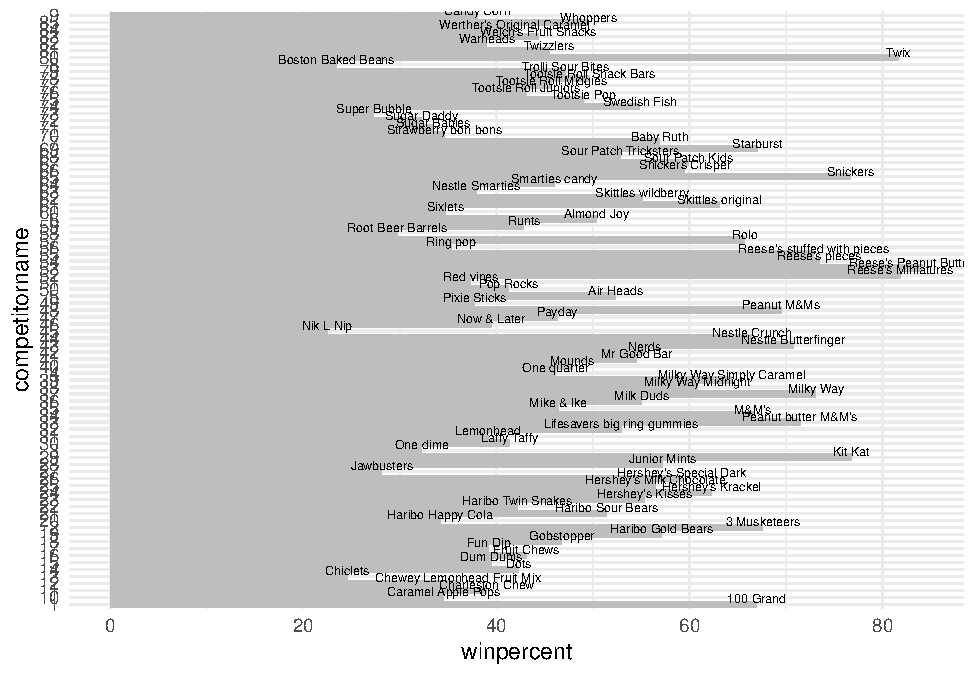
\includegraphics{Untitled_files/figure-latex/unnamed-chunk-17-1.pdf}
Q16. This is quite ugly, use the reorder() function to get the bars
sorted by winpercent?

\begin{Shaded}
\begin{Highlighting}[]
\FunctionTok{library}\NormalTok{(ggplot2)}

\FunctionTok{ggplot}\NormalTok{(candy\_file) }\SpecialCharTok{+} 
  \FunctionTok{aes}\NormalTok{(}\AttributeTok{x =}\NormalTok{ winpercent, }\AttributeTok{y =} \FunctionTok{rownames}\NormalTok{(candy\_file)) }\SpecialCharTok{+}
  \FunctionTok{geom\_bar}\NormalTok{(}\AttributeTok{stat =} \StringTok{"identity"}\NormalTok{, }\AttributeTok{fill =} \StringTok{"grey"}\NormalTok{) }\SpecialCharTok{+}
  \FunctionTok{labs}\NormalTok{(}\AttributeTok{x =} \StringTok{"winpercent"}\NormalTok{, }\AttributeTok{y =} \StringTok{"competitorname"}\NormalTok{) }\SpecialCharTok{+}
  \FunctionTok{geom\_text}\NormalTok{(}\FunctionTok{aes}\NormalTok{(}\AttributeTok{label=}\NormalTok{competitorname), }\AttributeTok{vjust=}\SpecialCharTok{{-}}\DecValTok{2}\NormalTok{, }\AttributeTok{size=}\DecValTok{1}\NormalTok{) }\SpecialCharTok{+}
  \FunctionTok{theme\_minimal}\NormalTok{() }\SpecialCharTok{+} \FunctionTok{aes}\NormalTok{(winpercent, }\FunctionTok{reorder}\NormalTok{(}\FunctionTok{rownames}\NormalTok{(candy\_file),winpercent))}
\end{Highlighting}
\end{Shaded}

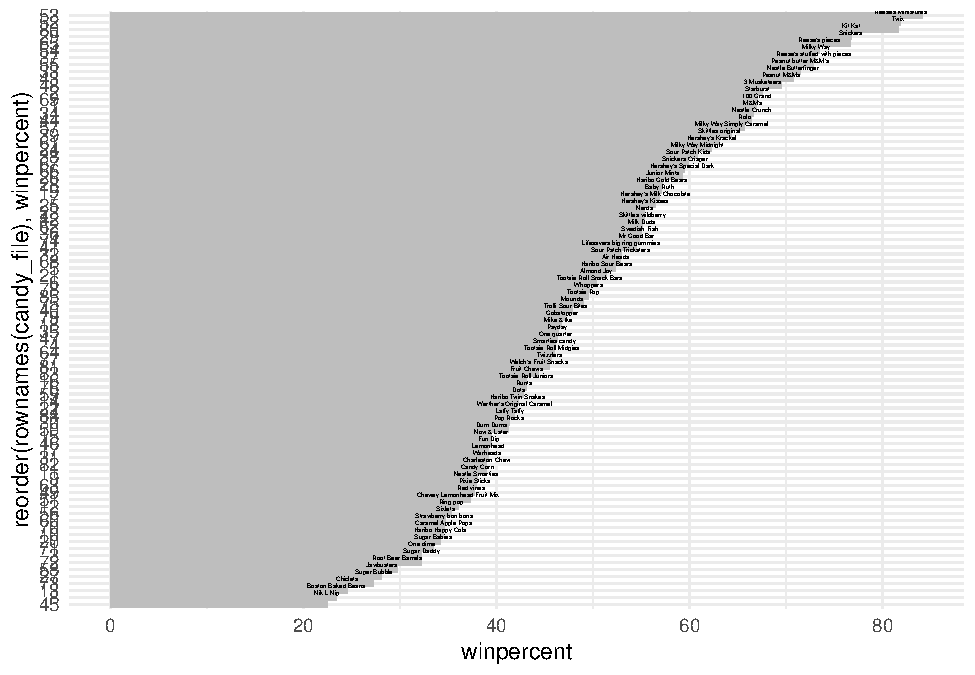
\includegraphics{Untitled_files/figure-latex/unnamed-chunk-18-1.pdf}

\begin{Shaded}
\begin{Highlighting}[]
\NormalTok{candy }\OtherTok{\textless{}{-}}\NormalTok{ candy\_file}
\NormalTok{my\_cols}\OtherTok{=}\FunctionTok{rep}\NormalTok{(}\StringTok{"black"}\NormalTok{, }\FunctionTok{nrow}\NormalTok{(candy))}
\NormalTok{my\_cols[}\FunctionTok{as.logical}\NormalTok{(candy}\SpecialCharTok{$}\NormalTok{chocolate)] }\OtherTok{=} \StringTok{"chocolate"}
\NormalTok{my\_cols[}\FunctionTok{as.logical}\NormalTok{(candy}\SpecialCharTok{$}\NormalTok{bar)] }\OtherTok{=} \StringTok{"brown"}
\NormalTok{my\_cols[}\FunctionTok{as.logical}\NormalTok{(candy}\SpecialCharTok{$}\NormalTok{fruity)] }\OtherTok{=} \StringTok{"pink"}

\FunctionTok{ggplot}\NormalTok{(candy) }\SpecialCharTok{+} 
  \FunctionTok{aes}\NormalTok{(}\AttributeTok{x =}\NormalTok{ winpercent, }\AttributeTok{y =} \FunctionTok{rownames}\NormalTok{(candy)) }\SpecialCharTok{+}
  \FunctionTok{geom\_bar}\NormalTok{(}\AttributeTok{stat =} \StringTok{"identity"}\NormalTok{, }\AttributeTok{fill =} \StringTok{"grey"}\NormalTok{) }\SpecialCharTok{+}
  \FunctionTok{labs}\NormalTok{(}\AttributeTok{x =} \StringTok{"winpercent"}\NormalTok{, }\AttributeTok{y =} \StringTok{"competitorname"}\NormalTok{) }\SpecialCharTok{+}
  \FunctionTok{geom\_text}\NormalTok{(}\FunctionTok{aes}\NormalTok{(}\AttributeTok{label=}\NormalTok{competitorname), }\AttributeTok{vjust=}\SpecialCharTok{{-}}\DecValTok{2}\NormalTok{, }\AttributeTok{size=}\DecValTok{1}\NormalTok{) }\SpecialCharTok{+}
  \FunctionTok{theme\_minimal}\NormalTok{() }\SpecialCharTok{+} \FunctionTok{aes}\NormalTok{(winpercent, }\FunctionTok{reorder}\NormalTok{(}\FunctionTok{rownames}\NormalTok{(candy),winpercent)) }\SpecialCharTok{+} \FunctionTok{geom\_col}\NormalTok{(}\AttributeTok{fill=}\NormalTok{my\_cols)}
\end{Highlighting}
\end{Shaded}

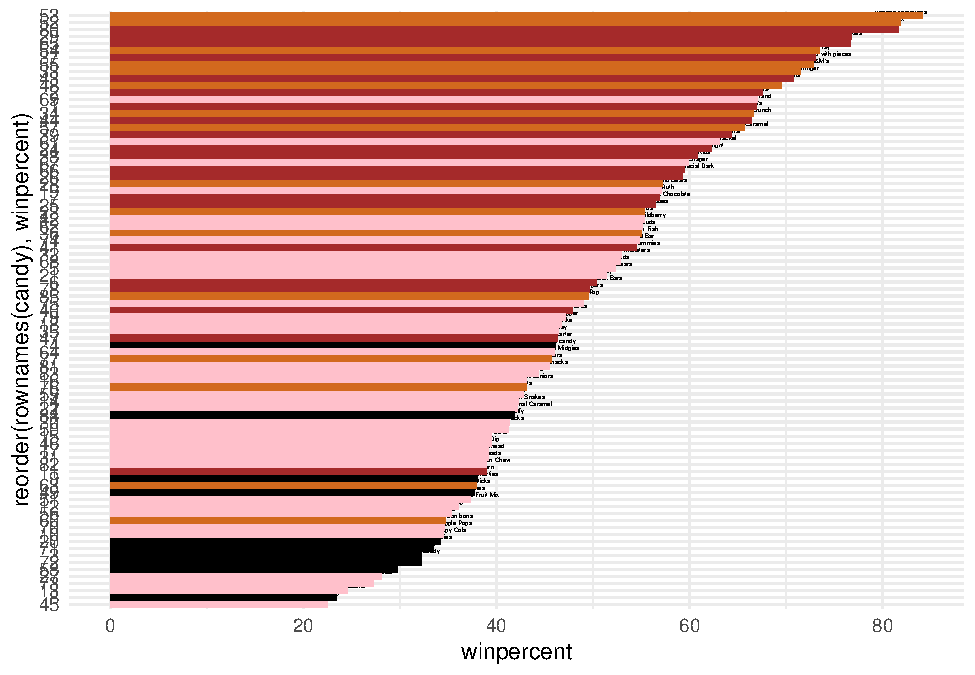
\includegraphics{Untitled_files/figure-latex/unnamed-chunk-19-1.pdf}
Q17. What is the worst ranked chocolate candy? The worst ranked
chocolate candy is Sixlets.

Q18. What is the best ranked fruity candy? The best ranked fruity candy
is Starburst.

\end{document}
